\section{Планирование цены и прогнозирование прибыли}

На основе рассчитанных затрат на изготовление и внедрение программного
продукта, а также результатов исследования рынка, необходимо
определить экономически обоснованную цену одной копии продукта и
оценить ожидаемую прибыль от его реализации.

Стоимость программного продукта определяется с учётом части затрат на
разработку, приходящейся на одну копию, затрат на внедрение и
заложенной прибыли. Расчёт выполняется по формуле:

\begin{equation}
K_{\text{по}} = (\Delta K + K_{\text{вн}})\cdot(1 + D_{\text{приб}}),
\end{equation}

где $\Delta K$ --- часть стоимости разработки, приходящаяся на одну
копию продукта; $K_{\text{вн}}$ --- стоимость внедрения одной копии;
$D_{\text{приб}}$ --- доля прибыли, заложенная в цену.

Частичная стоимость разработки одной копии определяется по формуле:

\begin{equation}
\Delta K = \frac{K}{N_p^o}\cdot(1 + H_{\text{ст}}),
\end{equation}

где $K$ --- затраты на изготовление продукта;
$N_p^o$ --- планируемое число продаж за расчётный период;
$H_{\text{ст}}$ --- ставка банковского процента по долгосрочному
кредиту.

Так как оценка прибыльности проводится на горизонте двух лет, при
планируемом объёме продаж 15 копий в год примем:

\[
N_p^o = 30 \text{ копий}.
\]

Из предыдущих расчётов:

\[
K = 1443246.44 \text{ руб.}, \qquad
K_{\text{вн,общ}} = 2539632.90 \text{ руб.}, \qquad
H_{\text{ст}} = 0.25.
\]

Тогда часть затрат на изготовление, приходящаяся на одну копию,
составит:

\[
\Delta K =
\frac{1443246.44}{30}\cdot 1.25 \approx 60135.27 \text{ руб.}
\]

Стоимость внедрения одной копии определяется как:

\[
K_{\text{вн}} =
\frac{2539632.90}{30} \approx 84654.43 \text{ руб.}
\]

Следовательно, полная себестоимость одной копии продукта составляет:

\begin{equation}
K_{\text{себ}} = \Delta K + K_{\text{вн}} =
60135.27 + 84654.43 = 144789.70 \text{ руб.}
\end{equation}

С учётом принятой рыночной цены одной копии:

\[
K_{\text{пр}} = 250000 \text{ руб.},
\]

можно определить долю прибыли:

\begin{equation}
D_{\text{приб}} =
\left(\frac{K_{\text{пр}}}{K_{\text{себ}}} - 1\right).
\end{equation}

Подставляя значения, получаем:

\[
D_{\text{приб}} =
\left(\frac{250000}{144789.70} - 1\right) \approx 0.726,
\]

или в процентном выражении:

\[
D_{\text{приб}} \approx 72.6\%.
\]

Полученное значение является более реалистичным для
узкоспециализированного программного продукта, ориентированного на
корпоративный рынок. Такая норма прибыли учитывает как необходимость
окупаемости затрат на разработку и внедрение, так и ограниченный объём
рынка.

Прибыль от реализации одной копии определяется по формуле:

\begin{equation}
C_{\text{приб}} = K_{\text{пр}} \cdot D_{\text{приб}} \cdot
(1 - H_{\text{ндс}}),
\end{equation}

где $H_{\text{ндс}} = 0.2$ --- ставка налога на добавленную стоимость.

Тогда прибыль от реализации одной копии составит:

\[
C_{\text{приб}} =
250000 \cdot 0.726 \cdot 0.8 \approx 145200 \text{ руб.}
\]

Годовая выручка при реализации 15 копий составит:

\[
V = 15 \cdot 250000 = 3750000 \text{ руб.}
\]

За два года выручка составит:

\[
V_2 = 30 \cdot 250000 = 7500000 \text{ руб.}
\]

Годовая прибыль при реализации 15 копий составит:

\[
C_{\text{год}} = 15 \cdot 145200 = 2178000 \text{ руб.}
\]

За два года:

\[
C_2 = 30 \cdot 145200 = 4356000 \text{ руб.}
\]

Для оценки изменения денежных потоков во времени составим фрагмент общего
баланса проекта с учётом выполненных расчётов. Расчётный период разобьём на
кварталы. Для более реалистичного отражения динамики продаж учтём, что в первые
месяцы проект находится на стадии завершения разработки и подготовки к
внедрению. В связи с этим в первые 3 месяца осуществляется только одна продажа,
после чего продажи стабилизируются. Предположим, что далее продажи
распределяются равномерно, и за оставшиеся периоды реализуется оставшийся объём
продукта.

Расчёт показателей таблицы~\ref{tab:balance} выполняется последовательно
для каждого расчётного периода.

Для $i$-го периода используются следующие зависимости:

\begin{itemize}
\item сумма продаж:
\begin{equation}
V_i = n_i \cdot K_{\text{пр}},
\end{equation}
где $n_i$ --- количество проданных копий в периоде;

\item затраты на внедрение:
\begin{equation}
C_{\text{вн},i} = n_i \cdot K_{\text{вн}},
\end{equation}

\item погашение затрат на разработку:
\begin{equation}
C_{\text{разр},i} = n_i \cdot \Delta K,
\end{equation}

\item чистая прибыль:
\begin{equation}
P_i = n_i \cdot C_{\text{приб}},
\end{equation}

\item конечный баланс:
\begin{equation}
B_i = B_{i-1} + P_i,
\end{equation}
где $B_{i-1}$ --- баланс на начало периода.
\end{itemize}

Рассмотрим пример расчёта для периода «4--6 месяцев», в котором
реализуется $n_2 = 3$ копии продукта.

Сумма продаж:
\[
V_2 = 3 \cdot 250000 = 750000 \text{ руб.}
\]

Затраты на внедрение:
\[
C_{\text{вн},2} = 3 \cdot 84654.43 = 253963.29 \text{ руб.}
\]

Погашение затрат на разработку:
\[
C_{\text{разр},2} = 3 \cdot 60135.27 = 180405.81 \text{ руб.}
\]

Чистая прибыль:
\[
P_2 = 3 \cdot 105210.30 = 315630.89 \text{ руб.}
\]

Баланс на начало периода:
\[
B_1 = -1338036.14 \text{ руб.}
\]

Тогда конечный баланс:
\[
B_2 = -1338036.14 + 315630.89 = -1022405.25 \text{ руб.}
\]

Аналогичным образом выполняются расчёты для остальных периодов.

\begin{table}[h]
\centering
\caption{Фрагмент общего баланса проекта с учётом выполненных расчётов}
\label{tab:balance}
\resizebox{\textwidth}{!}{
\begin{tabular}{|c|c|c|c|c|c|c|}
\hline
Период расчёта &
Баланс начальный, руб. &
Сумма продаж, руб. &
Сумма погашения кредита на внедрение, руб. &
Погашение кредита на разработку, руб. &
Чистая прибыль, руб. &
Баланс конечный, руб. \\ \hline

1--3 мес. &
$-1443246.44$ &
$250000.00$ &
$84654.43$ &
$60135.27$ &
$105210.30$ &
$-1338036.14$ \\ \hline

4--6 мес. &
$-1338036.14$ &
$750000.00$ &
$253963.29$ &
$180405.81$ &
$315630.89$ &
$-1022405.25$ \\ \hline

7--9 мес. &
$-1022405.25$ &
$1000000.00$ &
$338617.72$ &
$240541.08$ &
$420841.19$ &
$-601564.06$ \\ \hline

10--12 мес. &
$-601564.06$ &
$1000000.00$ &
$338617.72$ &
$240541.08$ &
$420841.19$ &
$-180722.87$ \\ \hline

13--15 мес. &
$-180722.87$ &
$1000000.00$ &
$338617.72$ &
$240541.08$ &
$420841.19$ &
$240118.32$ \\ \hline

16--18 мес. &
$240118.32$ &
$1000000.00$ &
$338617.72$ &
$240541.08$ &
$420841.19$ &
$660959.51$ \\ \hline

19--21 мес. &
$660959.51$ &
$1250000.00$ &
$423272.15$ &
$300676.35$ &
$526051.48$ &
$1187010.99$ \\ \hline

22--24 мес. &
$1187010.99$ &
$1250000.00$ &
$423272.15$ &
$300676.35$ &
$526051.49$ &
$1713062.48$ \\ \hline

\end{tabular}
}
\end{table}

Как видно из таблицы~\ref{tab:balance}, в первые три месяца проект
остаётся убыточным, что связано с завершением разработки и началом
внедрения, вследствие чего в данный период реализуется только одна
копия продукта. В последующие периоды объём продаж возрастает, а
проект достигает точки безубыточности к концу первого года
эксплуатации.

Дальнейшее увеличение количества продаж обеспечивает устойчивый рост
прибыли, что подтверждает экономическую целесообразность реализации
проекта при выбранной цене продукта.

Для наглядного представления динамики прибыли может быть построен
график изменения баланса и чистой прибыли по расчётным периодам.

\begin{figure}
\centering
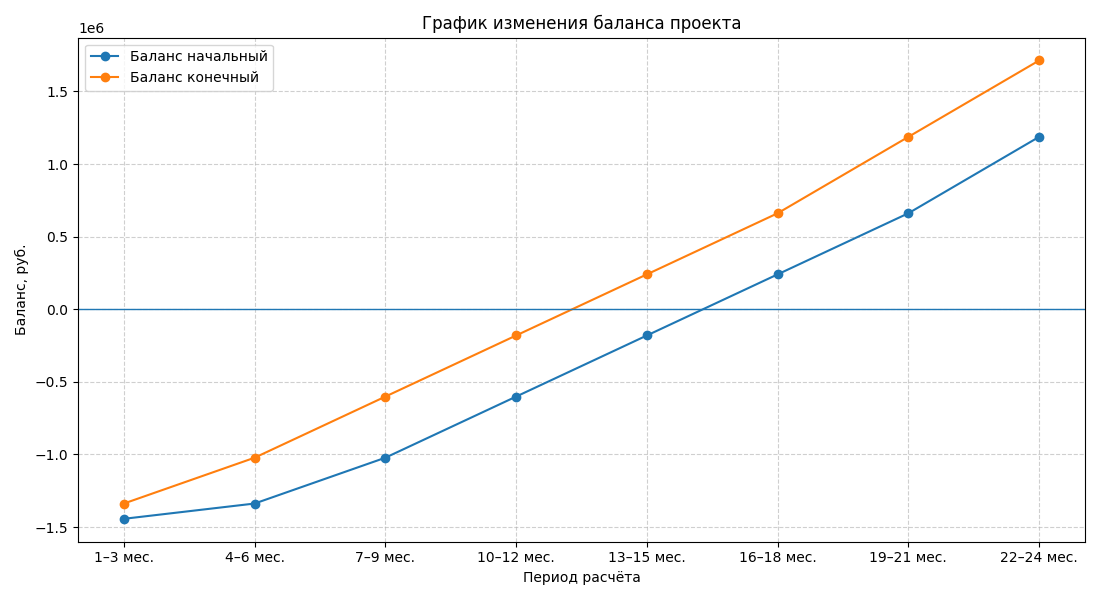
\includegraphics[width=0.75\textwidth]{inc/profit_balance.png}
\caption{График изменения баланса проекта}
\label{fig:profit_balance}
\end{figure}

Таким образом, выбранная цена продукта в размере 250000 руб.
обеспечивает покрытие затрат на изготовление и внедрение проекта и
позволяет получить положительный финансовый результат на горизонте
двух лет. При этом уровень прибыли остаётся умеренным и выглядит
более реалистично для специализированного программного продукта,
ориентированного на ограниченный сегмент рынка.
